    \begin{figure}\normalsize
    
    %\textbf{
    %    Intepretation}
    %\vspace{1em}

    %\begin{subfigure}%{.3\textwidth}
        \centering
        %\begin{scaletikzpicturetowidth}{\textwidth}
        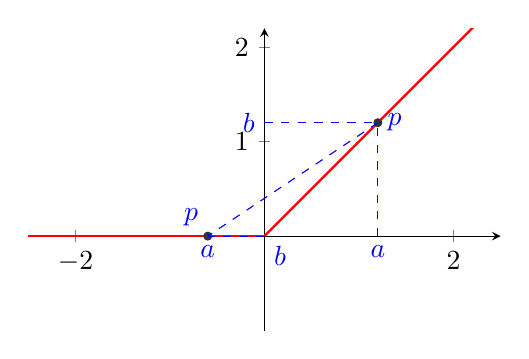
\begin{tikzpicture}
            \begin{axis}[
                axis lines=middle,
                y=1.2cm,
                x=1.2cm,
                xmax=2.5,
                xmin=-2.5,
                xtick={-2,0, 2},
                ymin=-1,
                ymax=2.2,
                ytick={0,1, 2},
                width=2cm
            ]
        
        
            \addplot [domain=-10:0, samples=100,
                      thick, red] {0};
                
            \addplot [domain=0:10, samples=100,
            thick, red] {x};

            \node at (axis cs:-0.6,0) [circle, scale=0.3, draw=black!80,fill=black!80] {};
            \node at (axis cs:1.2,1.2) [circle, scale=0.3, draw=black!80,fill=black!80] {};

            %\addplot[domain=0:1.2, dashed, color=blue] {1.2};
            \tikzstyle{dashed}=[dash pattern=on 3pt off 3pt,color=blue]
            \draw[dashed] (0,1.2) node[left] {$b$} -- (1.2,1.2) node[right] {$p$};
            \draw[dashed] (1.2,0) node[below] {$a$} -- (1.2,1.2) node[right] {};
            \draw[dashed] (1.2,1.2) node[below] {} -- (-0.6,0) node[right] {};
            \draw[dashed] (0,0) node[below right] {$\Tilde{b}$} -- (-0.6, 0) node[above left] {$\Tilde{p}$};
            \draw[dashed] (-0.6, 0) node[below] {$\Tilde{a}$};
            \addplot[mark=none, dashed, color=blue] coordinates {(1.2, 0) (1.2, 1.2)};
            %\addplot+[sharp plot, color=blue] coordinates {(-0.5,0) (1.2,0) (1.2,1.2) } node[below=0.5mm, pos=-0.01,color=blue] {$x_1$}
    %node[below=15mm,color=blue] {$x_2$}
    %node[above=0.5mm,color=blue] {$y_2$};
        
        \end{axis}
        \end{tikzpicture}
        %\end{scaletikzpicturetowidth}
        \[ \relu(x) = \left\{ \begin{array}{ll}
            x, & \mbox{$x \geq 0$}\\
            0, & \mbox{$x < 0$}\end{array} \right. 
        \]
        \caption{An illustration of the $\relu$ function. $p$ and $\Tilde{p}$ are on the two different branches of $\relu$. The slope between any two points on the function is always within $[0,1]$.}\label{fig:relu}
        %\end{subfigure}
        \end{figure}